\documentclass{article}
\usepackage{graphicx}
\usepackage{subfigure}
%\usepackage{subfig}
\begin{document}
\section{Tag Frequency Diagrams}
\subsection{Experiment Setup}
\paragraph{The Input Blocks of Tags}
In this experiment, the length of a input block, D, to CETD is 16 bits.The hexadecimal domain of D block is [0x0000, 0xFFFF].  The tag length is set to 8 bits, so the input block D is splited into two sub-blocks D$_a$ and D$_b$. Each sub-block has a length of 8 bits.

Our experiment simulate the replay attack. Using each distinct value in the domain of D as input to CETD, we generated 1000 tags. For the input of nonce for each tag, the following two principles is met:
\begin{itemize}
	\item The counter is distinct
	\item The random number is randomly generated by PRF
\end{itemize}
Hence the block cipher we use in nonce generation is AES, each nonce in the 1000 times tag generation is randomly generated. 
We want to examine the distribution of distinct tag values for each distinct D block. 
\begin{figure}[htbp]
 \centering
 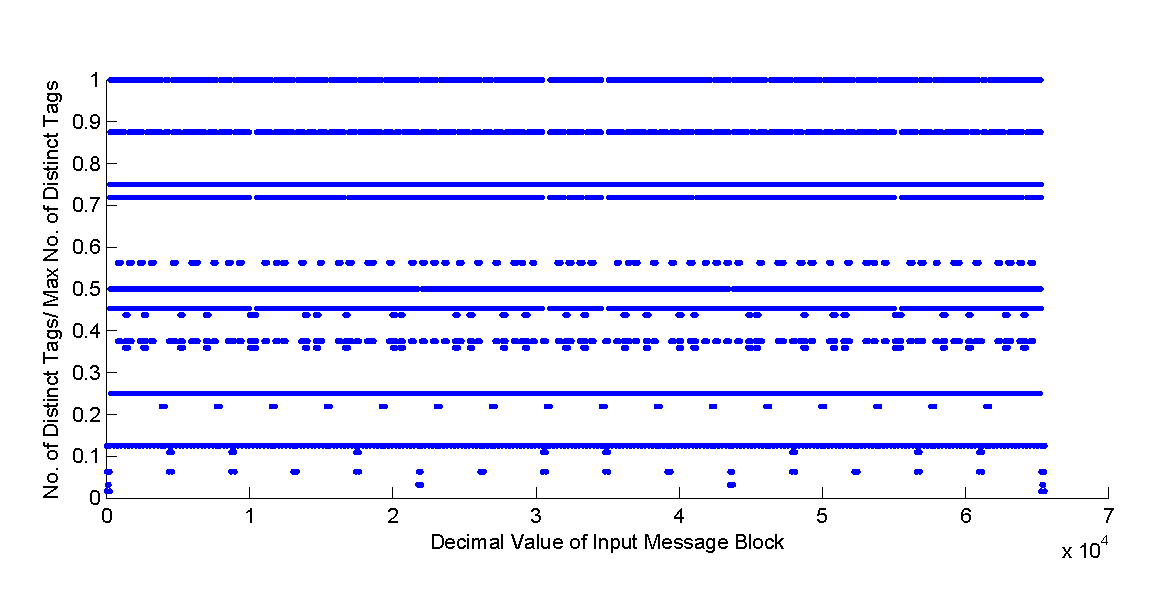
\includegraphics[scale=0.4]{./frequency/overall_frequency_spot.pdf}
 \caption{The tag value frequency diagram for all D blocks. Y axis expresses the frequency of tag values of a D value divided by the maximum frequecy}
 \label{fig:1 }
\end{figure} 

\begin{figure}[htbp]
 \centering
 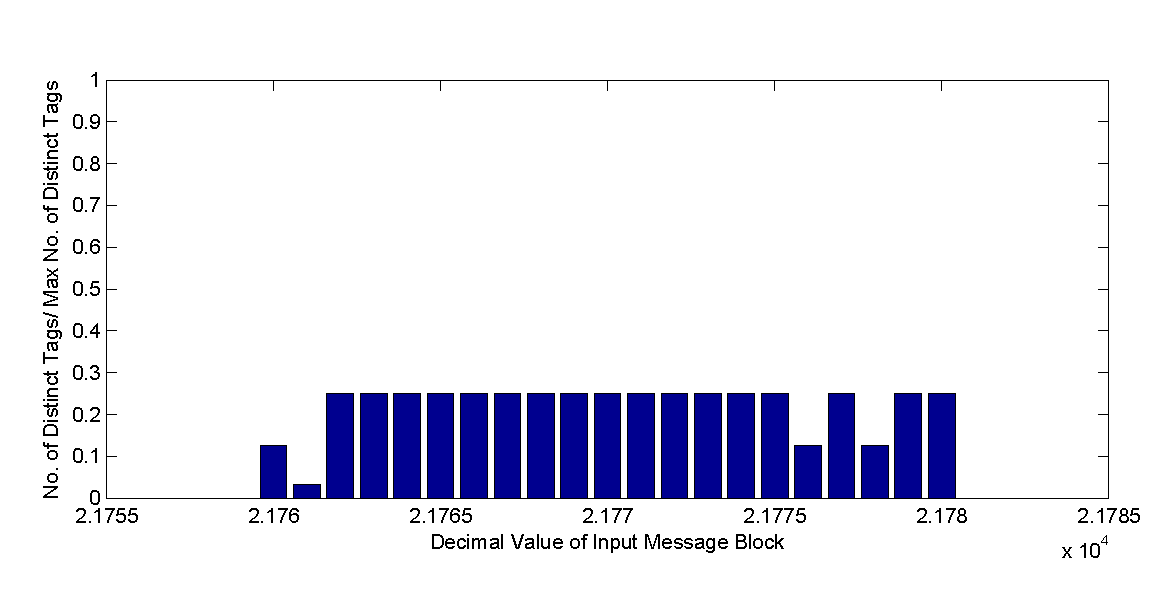
\includegraphics[scale=0.4]{./frequency/portion_bar.pdf}
 \caption{The tag value frequency diagram for a part of D blocks}
 \label{fig:2 }
\end{figure} 


\subsection{The Results}
\paragraph{The Frequency Diagram of All D Values}
The tag frequency diagram of all D values is expressed in Figure 1. From the figure we can see that the frequency of tag varies to different levels. Figure enlarge a part of Figure 1 to help clarify the tag frequency of each D block. 

\begin{figure}[htbp]
 \centering
 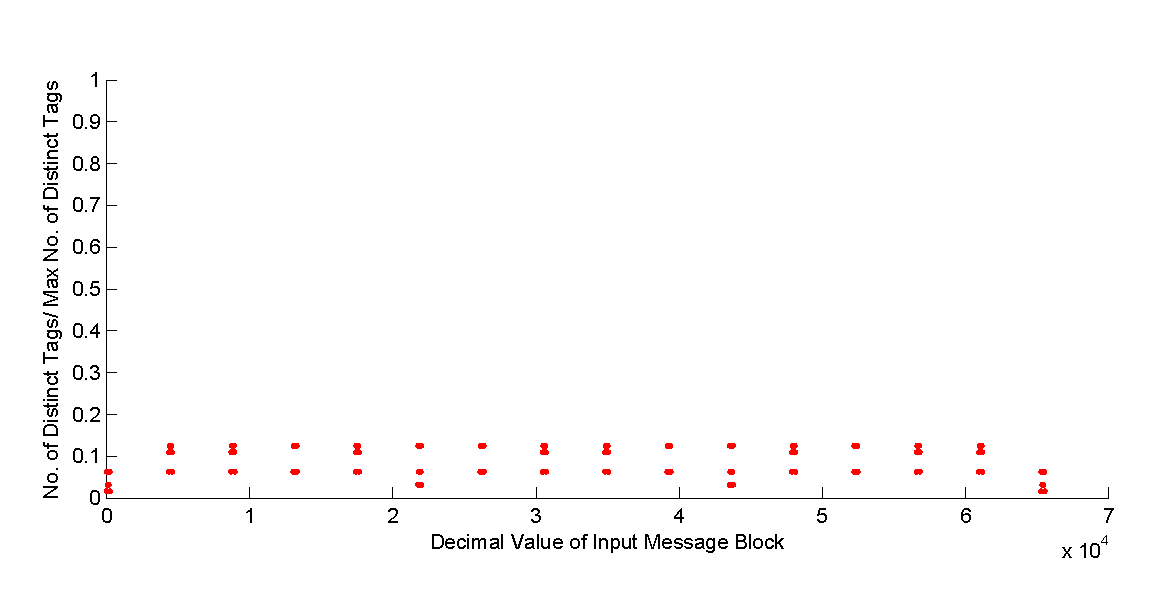
\includegraphics[scale=0.4]{./frequency/pattern_frequency_spot.pdf}
 \caption{The tag value frequency diagram for D blocks formed by pattern sub-blocks. }
 \label{fig:3}
\end{figure}
\paragraph{The Frequency Diagram of D Values formed by Pattern Sub-blocks}
As analyzed before, the tag has more probability to collide under replay attack if each sub-block of D is formed by a pattern. We found all the D values formed by two pattern sub-blocks. Figure 2 expresses the tag frequncy values of these D blocks.

We can see that the tag frequency of all D blocks formed by pattern sub-blocks is small. These points on the Fig 3 exactly match the lowest points in Fig 1. 
\end{document}